
\chapter{Example Comparison to Observational Data}
\label{bursts:appendix:obs_compare}
In this section, we demonstrate a comparison between model predictions as 
calculated by~\texttt{VICE} and observational data, taking the catalog of 
stars in Milky Way dwarf satellite galaxies from~\citet{Kirby2010} as an 
example. We clarify that we are not modeling the observational data in detail 
to derive conclusions about how these dwarf galaxies evolved, but rather 
illustrate how one might go about using \texttt{VICE} to do so as well as to 
connect the results presented in this work to what is observed in nature. 
\par 
The~\citet{Kirby2010} sample consists of 2961 stars from eight dwarf satellite 
galaxies of the Milky Way: Sculptor, Fornax, Leo I, Sextans, Leo II, Canes 
Ventatici I, Ursa Minor, and Draco. They derive abundances of Fe, Mg, Si, Ca, 
and Ti through Keck/DEIMOS medium-resolution spectroscopy combined with 
spectral synthesis. For demonstration purposes, we cut the sample by removing 
all stars that do not have measurements for all five of these elements, 
resulting a sample of 849 stars. Our final sample thus consists of stars from 
each of these dwarf galaxies with the exception of Fornax, for which no star 
meets this requirement. 
\par 
In Fig.~\ref{bursts:fig:kirby2010}, we plot this sample in the [Mg/Fe]-[Fe/H] plane. 
These stars are at significantly subsolar metallicities, which is expected 
given the low stellar masses of these galaxies and the observed 
mass-metallicity relation~\citep[e.g.][]{Andrews2013}. The error bars in the 
lower-left corner illustrate the median uncertainties in [Fe/H] and [Mg/Fe] 
for the Ursa Minor sample. This demonstrates that a signifcant portion of the 
scatter in these data is due to large observational uncertainties. In 
principle, there should also be
some level of physical scatter 
due to the timescale for mixing of newly produced metals in the ISM, an 
effect which is deliberately neglected by the instantaneous mixing 
approximation. 
Different dwarfs could also be offset because of differences in 
star formation efficiency, outflows, etc.

\begin{figure} % Fig 12 
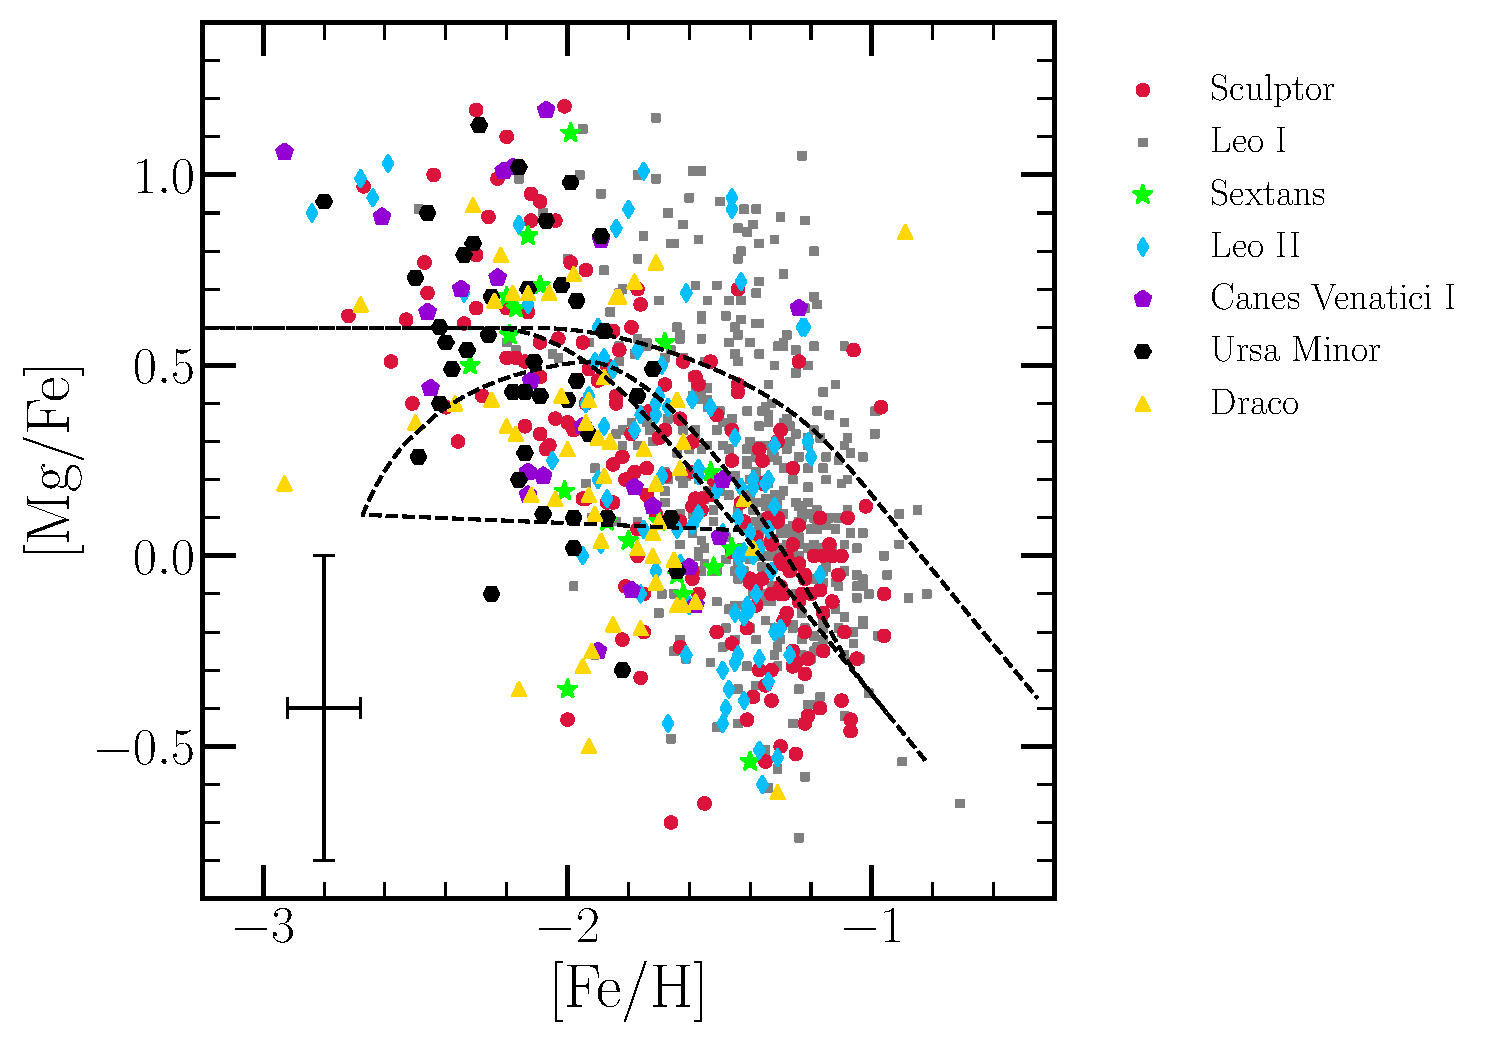
\includegraphics[scale = 0.34]{./chapter2/kirby2010.pdf} 
\caption{
A comparison of three chemical evolution models simulated by~\texttt{VICE} to 
the data obtained by~\citet{Kirby2010}. All model predictions are plotted in a 
dashed black line, while the colored points with various symbols correspond to 
various dwarf galaxies as indicated by the legend. The error bar in the lower 
left shows the median error in [Fe/H] and the median error in [Mg/Fe] for the 
Ursa Minor sample. The model prediction with the highest final [Fe/H] 
corresponds to one with an initial ISM mass of 0 $M_\odot$, an exponential 
infall history with e-folding timescale $\tau_\text{in}$ = 2 Gyr 
($\dot{M}_\text{in} = 9.1\ M_\odot\ \text{yr}^{-1}$ at $t = 0$), SFE 
timescale of $\tau_*$ = 10 Gyr, and mass loading factor $\eta$ = 30. The 
lower-metallicity models correspond to the same parameters with an outflow 
enhancement factor $\xi_\text{enh}$ = 3 (i.e. $Z_\text{outflow} = 
3Z_\text{ISM}$). The third and final model is one in which $5\times10^9\ 
M_\odot$ of $Z$ = 0 gas is added at $t = 5$ Gyr, similar to the gas-driven 
starburst models explored in the top panel of Fig.~\ref{bursts:fig:fiducial_cases}. 
}
\label{bursts:fig:kirby2010} 
\end{figure} 

While the~\citet{Kirby2010} sample does not provide abundances of O, which our 
analysis has focused on thus far as the representative $\alpha$ element, 
Mg is also an $\alpha$ element and can be interpreted similarly. We 
therefore adopt $y_\text{Mg}^\text{Ia}$ = 0 similar to O, and a value of 
$y_\text{Mg}^\text{CC}$ such that [Mg/Fe] = 0.6 at low [Fe/H]. In that regime, 
[Mg/Fe] is set by the ratio of yields from CCSN-dominated enrichment, namely: 
\begin{equation} 
\text{[Mg/Fe]}_\text{CC} = \log_{10}\left(\ddfrac{y_\text{Mg}^\text{CC}}
{y_\text{Fe}^\text{CC}}\right) - \log_{10}\left(\ddfrac{Z_{\text{Mg,}\odot}}
{Z_{\text{Fe,}\odot}}\right), 
\end{equation} 
where the yields are again defined by equation~\refp{bursts:eq:frac_yield}. 
By specifying [Mg/Fe]$_\text{CC}$ = 0.6, adopting $y_\text{Fe}^\text{CC}$ = 
0.0012 as in this work, and the solar abundances measured 
by~\citet{Asplund2009}, this equation dictates $y_\text{Mg}^\text{CC}$ = 
0.00261. This value is not calculated using yield tables from supernova 
nucleosynthesis studies as in previous sections, and is instead adopted in the 
interest of obtaining a simple model which may accurately describe these 
galaxies. 
\par 
We next define a one-zone chemical evolution model with an initial ISM mass of 
0 $M_\odot$, an exponential infall history with e-folding timescale 
$\tau_\text{in}$ = 2 Gyr, SFE timescale $\tau_*$ = 10 Gyr, and mass-loading 
factor $\eta$ = 30. This model is plotted over the~\citet{Kirby2010} sample in 
Fig.~\ref{bursts:fig:kirby2010}, and extends to higher [Fe/H] than the observational 
sample. We then modify this model with an outflow enhancement factor 
$\xi_\text{enh}$ = 3 (i.e. the outflows are 3 times the metallicity of the 
ISM), motivated by the observations of~\citet{Chisholm2018} which suggest 
that dwarf galaxies have metal-rich outflows relative to their interstellar 
media. This model reaches lower [Fe/H] at late times and slightly lower 
[Mg/Fe], in better agreement with the data from all of these galaxies. 
The metal-weighted outflow mass-loading required to achieve this agreement,
$\xi_{\rm enh}\eta = 90$, is high.
However, it is a plausible extrapolation of the mass/metal-loading trends
required to match, e.g., the observed mass-metallicity relation
\citep{Finlator2008,Peeples2011} to the mass range
$M_* \sim 10^6-10^7 M_\odot$ of the dwarfs.
\par
We further modify this model to exhibit a starburst at $t = 5$ Gyr in a similar 
manner as the models explored in the top row of Fig.~\ref{bursts:fig:fiducial_cases}, 
namely: 
\begin{equation} 
\dot{M}_\text{in} = \begin{cases} 
5000\ M_\odot\ yr^{-1} & (5\text{ Gyr} < t < 5.001\text{ Gyr}) \\ 
9.1e^{-t / (\text{2 Gyr})}\ M_\odot\ yr^{-1} & \text{otherwise}. 
\end{cases} 
\label{bursts:eq:kirby2010_burst_model}
\end{equation} 
This produces the jump-and-hook trajectory seen in Fig.~\ref{bursts:fig:kirby2010} 
whose details are discussed in~\S~\ref{bursts:sec:gas-driven}. 
\par 
Due to the associated observational uncertainties, it is not immediately 
obvious from this figure whether any of these galaxies experienced a starburst 
accurately described by this model. A more detailed investigation would 
compare model predictions of stellar abundance and age distributions to the 
observed data, quantifying the relative likelihoods of various models with and 
without starbursts to constrain their evolutionary histories. 
